\scanpage{121}
\mspage{6}

Je vais donner \deleted{6} \inserted{trois} autres présentations, où on élimine non seulement les pts proches (disons) des \deleted{$\unsure{R_q}$} sommets de type $\infty$, \inserted{et les sommets qui leur sont liés \unsure{d'indice|d'arc} $\infty$} mais aussi ceux proches des sommets (disons) de type $1$, en gardant donc que les sommets \inserted{$R_r^{ij}$} de type $0$, i.e.
\[
(20)\qquad R_r^{0,1}\ \swarrow\qquad r\in\mathcal{R}
\]
\margin{$\boxed{R_r^{0,1}=R_{\unsure{\sigma_\infty r|\tau_\infty r}}^{01}}$

relations de redondance pour mémoire}
et on introduit les chemins
\[
(21)\qquad\left\{\begin{aligned}
A_r^{0,1}&\overset{\text{déf}}{=}(a_{\tau_0r}^\infty)^{-1}(\unsure{\Lambda_r^{\prime1}|\Lambda_r^1})^{-1}a_r^\infty:R_r^{01}\longrightarrow R_{\unsure{\sigma_0(r)|\tau_0(r)}}^{0,1}\qquad(r\in\mathcal{R})\\
\Lambda_r^0&:R_r^{0,1}\mathrel{\unsure{-|\longrightarrow}} R_{\unsure{\sigma_1r|\tau_1r}}^{01}\qquad(r\in\mathcal{R})
\end{aligned}\right.
\]
\margin{plus les chemins déjà connus}
on a les relations de redondance
\[
(22)\qquad\boxed{\left\{\begin{aligned}
\Lambda_r^0\Lambda_{\unsure{\tau_1(r)|\sigma_1(r)}}^0&=1&&r\in\mathcal{R}\\
A_r^{0,1}A_{\unsure{\sigma_0(r)|\tau_0(r)}}^{0,1}&=1&&r\in\mathcal{R}
\end{aligned}\right.}
\]
\figure{
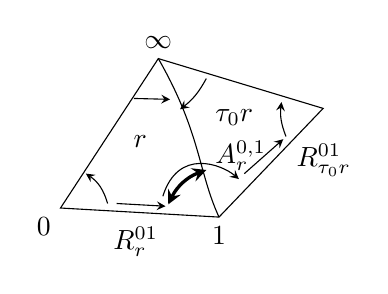
\begin{tikzpicture}[scale=1.15,>=stealth]
\coordinate (A) at (0,0);\coordinate (B) at (1.75,-0.10);\coordinate (C) at (1.08,1.65);\coordinate (D) at (2.90,1.10);
\draw (A)--(C)--(D)--(B)--cycle;
\draw (C)..controls(1.55,0.83)and(1.52,0.40)..(B);
\draw[->] (0.81,1.21)--(1.21,1.20);
\draw[->] (1.61,1.43) to[bend left=12] (1.32,1.09);
\draw[->] (0.52,0.05) to[bend right=20] (0.28,0.38);
\draw[->] (0.62,0.05)--(1.16,0.02);
\draw[very thick,<->] (1.19,0.04) to[bend left=22] (1.61,0.42);
\draw[->] (1.13,0.13)..controls(1.30,0.67)and(1.78,0.48)..(1.97,0.32);
\draw[->] (2.03,0.38)--(2.46,0.76);
\draw[->] (2.49,0.79) to[bend left=14] (2.44,1.17);
\node[below left] at (A) {$0$};\node[below] at (B) {$1$};\node[above] at (C) {$\infty$};
\node at (0.88,0.73) {$r$};\node at (1.92,1.00) {$\tau_0r$};\node at (1.99,0.58) {$A_r^{0,1}$};
\node[below] at (0.83,-0.10) {$R_r^{01}$};\node[right] at (2.50,0.53) {$R_{\tau_0r}^{01}$};
\end{tikzpicture}
}
et c'est tout : $\Pi_1(\widetilde{X}^{\substack{*\\*}*},\{R_r^{01}\}_{r\in\mathcal{R}})$ est \deleted{engendré} \inserted{présenté} par les sommets et flèches $(20)$ $(21)$, avec les seules relations de redondance $(20)$ $(22)$.

\uline{Bouchage \unsure{de|des} trous} Dans chacun des quatre cas envisagés, (en fait $10=1+3+3+3$ cas), le ``bouchage'' d'un trou $R_{\deleted{\unsure{q}}s}$ $(s\in S=S_0\amalg S_1\amalg S_\infty)$ se fait de façon essentiellement triviale. Dans chacun des quatre cas, il faut, en termes des flèches génératrices choisies, définir \unsure{\uline{les}|\deleted{les}}

\mspage{120}
